% Chapter 8: Optimization for Training Deep Models

\chapter{Optimization for Training Deep Models}
\label{chap:optimization}

This chapter covers optimization algorithms and strategies for training deep neural networks effectively. Modern optimizers go beyond basic gradient descent to accelerate convergence and improve performance.

\begin{learningobjectives}
\objective{Gradient descent variants and appropriate batch size selection}
\objective{Momentum-based methods including classical momentum and Nesterov accelerated gradient}
\objective{Adaptive optimizers (AdaGrad, RMSProp, Adam) and hyperparameter tuning}
\objective{Second-order approaches and when they are practical}
\objective{Optimization challenges and their remedies}
\objective{Optimization plan combining initializer, optimizer, and learning rate schedule}
\end{learningobjectives}




% Chapter 8, Section 1

\section{Gradient Descent Variants \difficultyInline{intermediate}}
\label{sec:gd-variants}

\subsection{Intuition: Following the Steepest Downhill Direction}

Imagine standing on a foggy hillside trying to reach the valley. You feel the slope under your feet and take a step downhill. \textbf{Batch gradient descent} measures the average slope using the whole landscape (dataset) before each step: accurate but slow to gauge. \textbf{Stochastic gradient descent (SGD)} feels the slope at a single point: fast, but noisy. \textbf{Mini-batch} is a compromise: feel the slope at a handful of nearby points to get a reliable yet efficient direction. This trade-off underlies most practical training regimes.\index{optimization!gradient descent}\index{mini-batch}\gls{mini-batch}

Historical note: Early neural network training widely used batch gradient descent, but the rise of large datasets and GPUs made mini-batch SGD the de facto standard \cite{GoodfellowEtAl2016,Prince2023}.

\subsection{Batch Gradient Descent}

Computes gradient using entire training set:
\begin{equation}
\vect{\theta}_{t+1} = \vect{\theta}_t - \alpha \nabla_{\vect{\theta}} \frac{1}{n} \sum_{i=1}^{n} L(\vect{\theta}, \vect{x}^{(i)}, y^{(i)})
\end{equation}

Characteristics:\index{gradient descent!batch}
\begin{itemize}
    \item Deterministic and low-variance updates; well-suited for convex problems.
    \item Each step uses all \(n\) examples, incurring high computation and memory costs for large datasets.
    \item In deep, non-convex landscapes, stable but often too slow to respond to curvature changes.
\end{itemize}

Example (convex quadratic): Let \(L(\theta)=\tfrac{1}{2}a\theta^2\) with gradient \(a\theta\). Batch GD with step size \(\alpha\) yields \(\theta_{t+1}=(1-\alpha a)\theta_t\). Convergence occurs if \(0<\alpha<\tfrac{2}{a}\), illustrating the learning-rate–curvature interaction.\index{learning rate}\glsadd{gradient-descent}

When to use:
\begin{itemize}
    \item Small datasets that fit comfortably in memory.
    \item Convex or nearly convex objectives (e.g., linear/logistic regression) when precise convergence is desired.
\end{itemize}

Historical context: Full-batch methods trace back to classical numerical optimization. For massive datasets, stochastic approximations dating to \cite{RobbinsMonro1951} became essential; modern deep learning typically favors mini-batches \cite{GoodfellowEtAl2016,WebOptimizationDLBook,D2LChapterOptimization}.

\subsection{Stochastic Gradient Descent (SGD)}\index{SGD@stochastic gradient descent}

Uses a single random example per update:
\begin{equation}
\vect{\theta}_{t+1} = \vect{\theta}_t - \alpha \nabla_{\vect{\theta}} L(\vect{\theta}, \vect{x}^{(i)}, y^{(i)})
\end{equation}

Characteristics:\glsadd{stochastic-gradient-descent}
\begin{itemize}
    \item Very fast, streaming-friendly updates; one pass can begin learning immediately.
    \item Noisy gradients add exploration, helping traverse saddle points and plateaus.\index{saddle point}\index{plateau}
    \item High variance can hamper precise convergence; diminishing \(\alpha_t\) helps stabilize \cite{RobbinsMonro1951}.
\end{itemize}

Practical tips:
\begin{itemize}
    \item Use a decaying schedule (e.g., \(\alpha_t = \alpha_0/(1+\lambda t)\)) or switch to momentum/Adam later for fine-tuning \cite{WebOptimizationDLBook,D2LChapterOptimization}.
    \item Shuffle examples every epoch to avoid periodic bias.
\end{itemize}

Applications: Early CNN training and many online/streaming scenarios employ SGD due to its simplicity and ability to handle large-scale data. In large vision models, SGD with momentum remains competitive \cite{He2016}.

\subsection{Mini-Batch Gradient Descent}\index{gradient descent!mini-batch}

Balances batch and stochastic approaches:
\begin{equation}
\vect{\theta}_{t+1} = \vect{\theta}_t - \alpha \nabla_{\vect{\theta}} \frac{1}{|\mathcal{B}|} \sum_{i \in \mathcal{B}} L(\vect{\theta}, \vect{x}^{(i)}, y^{(i)})
\end{equation}

where $\mathcal{B}$ is a mini-batch (typically 32–1024 examples depending on model and hardware).\glsadd{mini-batch}

Benefits:
\begin{itemize}
    \item Reduces gradient variance
    \item Efficient GPU utilization
    \item Good balance of speed and stability
\end{itemize}

Further guidance:
\begin{itemize}
    \item Larger batches yield smoother estimates but may require proportionally larger learning rates; the ``linear scaling rule'' is a useful heuristic in some regimes.\index{mini-batch}
    \item Very large batches can hurt generalization unless paired with warmup and appropriate regularization. See \cite{WebOptimizationDLBook,D2LChapterOptimization}.
\end{itemize}

Illustrative example (variance vs. batch size): For a fixed \(\alpha\), increasing \(|\mathcal{B}|\) reduces the variance of the stochastic gradient approximately as \(\mathcal{O}(1/|\mathcal{B}|)\), improving stability but diminishing returns once hardware is saturated.


% Chapter 8, Section 2

\section{Momentum-Based Methods \difficultyInline{intermediate}}
\label{sec:momentum}

\subsection{Intuition: Rolling a Ball Down a Valley}

Plain SGD can wobble like a marble on a bumpy path. \textbf{Momentum} acts like mass: it carries velocity so you keep moving in consistently good directions and smooth out small bumps. Imagine a heavy ball rolling down a hill—its mass (momentum) helps it maintain direction even when hitting small bumps, just like how momentum accumulates past gradients to maintain consistent movement in the loss landscape. The derivative of momentum with respect to time gives us the acceleration, but in optimization, we use the derivative of the loss with respect to parameters to determine the direction, while momentum provides the "inertia" to keep moving smoothly. \textbf{Nesterov acceleration} adds anticipation by peeking where the momentum will take you before correcting, often yielding crisper steps in curved valleys. Think of it like a skilled skier who looks ahead to anticipate the curve and adjusts their trajectory before reaching it, rather than just following their current momentum and then correcting afterward. This "look-ahead" approach helps the optimizer make more informed decisions by evaluating the gradient at the anticipated future position, leading to smoother and more efficient convergence.\index{momentum}\index{Nesterov}

Historical note: Momentum has deep roots in convex optimization and was popularized in early neural network training; Nesterov's variant provided stronger theoretical guarantees in convex settings and inspired practical variants in deep learning \cite{Polyak1964,Nesterov1983,GoodfellowEtAl2016,Bishop2006}.

\subsection{Momentum}

Accumulates gradients over time:
\begin{align}
\vect{v}_t &= \beta \vect{v}_{t-1} - \alpha \nabla_{\vect{\theta}} L(\vect{\theta}_t) \\
\vect{\theta}_{t+1} &= \vect{\theta}_t + \vect{v}_t
\end{align}

where $\beta \in [0, 1)$ is the momentum coefficient (typically 0.9).

Benefits:\index{optimization!momentum}
\begin{itemize}
    \item Accelerates convergence in relevant directions
    \item Dampens oscillations
    \item Helps escape local minima and saddle points
\end{itemize}

Interpretation: Momentum is equivalent to an exponentially weighted moving average of past gradients, implementing a low-pass filter that suppresses high-frequency noise. In anisotropic valleys, it allows larger effective step along the shallow curvature direction while reducing zig-zag across the sharp direction \cite{Polyak1964,WebOptimizationDLBook,D2LChapterOptimization}.

Choice of hyperparameters:
\begin{itemize}
    \item \(\beta\in[0.8,0.99]\); larger values increase smoothing and memory.
    \item Couple with a tuned \(\alpha\); too-large \(\alpha\) can still diverge.
\end{itemize}

Example (ravine function): For \(L(\theta_1,\theta_2)=100\theta_1^2+\theta_2^2\), momentum reduces oscillations in the steep \(\theta_1\) direction and speeds travel along the gentle \(\theta_2\) direction.

\subsection{Nesterov Accelerated Gradient (NAG)}\index{optimization!Nesterov}

"Look-ahead" version of momentum:
\begin{align}
\vect{v}_t &= \beta \vect{v}_{t-1} - \alpha \nabla_{\vect{\theta}} L(\vect{\theta}_t + \beta \vect{v}_{t-1}) \\
\vect{\theta}_{t+1} &= \vect{\theta}_t + \vect{v}_t
\end{align}

Evaluates gradient at anticipated future position, often providing better updates.

Rationale: By computing the gradient at the look-ahead point \(\theta_t+\beta v_{t-1}\), NAG corrects the course earlier, which reduces overshoot in curved valleys and can improve convergence rates in convex settings \cite{Nesterov1983,WebOptimizationDLBook,GoodfellowEtAl2016}.

Practice notes:
\begin{itemize}
    \item Common defaults: \(\beta=0.9\), initial \(\alpha\in[10^{-3},10^{-1}]\) depending on scale.
    \item Widely used with SGD in large-scale vision models \cite{He2016}.
    \item Start with \(\beta=0.9\) and tune \(\alpha\) based on your loss scale; for well-normalized networks, \(\alpha=0.01\) often works well.
    \item NAG typically requires fewer iterations than standard momentum to converge, making it particularly valuable for expensive training runs.
    \item The look-ahead gradient computation adds minimal computational overhead (one extra gradient evaluation per step) while often providing significant convergence improvements.
    \item Consider using NAG when training deep networks with many parameters, as the anticipation effect helps navigate complex loss landscapes more efficiently than standard momentum.
\end{itemize}


% Chapter 8, Section 3

\section{Adaptive Learning Rate Methods \difficultyInline{intermediate}}
\label{sec:adaptive-methods}

\subsection{Intuition: Per-Parameter Step Sizes}

Different parameters learn at different speeds: some directions are steep, others are flat. \textbf{Adaptive methods} adjust the step size per parameter based on recent gradient information, allowing faster progress on rarely-updated or low-variance dimensions while stabilizing steps on highly-volatile ones.\index{adaptive optimization}\index{AdaGrad}\index{RMSProp}\index{Adam}

Historical note: AdaGrad emerged for sparse problems; RMSProp stabilized AdaGrad's decay; Adam blended momentum with RMSProp-style adaptation and became a widely used default in deep learning \cite{Duchi2011,Tieleman2012,Kingma2014,GoodfellowEtAl2016}.

\subsection{AdaGrad}

Adapts learning rate per parameter based on historical gradients:
\begin{align}
\vect{g}_t &= \nabla_{\vect{\theta}} L(\vect{\theta}_t) \\
\vect{r}_t &= \vect{r}_{t-1} + \vect{g}_t \odot \vect{g}_t \\
\vect{\theta}_{t+1} &= \vect{\theta}_t - \frac{\alpha}{\sqrt{\vect{r}_t + \epsilon}} \odot \vect{g}_t
\end{align}

where $\epsilon$ (e.g., $10^{-8}$) prevents division by zero. AdaGrad is well-suited to sparse features: infrequent parameters receive larger effective steps, accelerating learning in NLP and recommender settings \cite{Duchi2011,WebOptimizationDLBook,D2LChapterOptimization}. A drawback is the ever-growing accumulator \(\vect{r}_t\), which can shrink steps too aggressively over long runs.

\subsection{RMSProp}

Addresses AdaGrad's aggressive decay using exponential moving average:
\begin{align}
\vect{r}_t &= \rho \vect{r}_{t-1} + (1-\rho) \vect{g}_t \odot \vect{g}_t \\
\vect{\theta}_{t+1} &= \vect{\theta}_t - \frac{\alpha}{\sqrt{\vect{r}_t + \epsilon}} \odot \vect{g}_t
\end{align}

Add a small \(\epsilon\) for numerical stability and tune decay \(\rho\in[0.9,0.99]\). RMSProp prevents the learning rate from decaying to zero as in AdaGrad, making it effective for non-stationary objectives typical in deep networks \cite{Tieleman2012,WebOptimizationDLBook,D2LChapterOptimization}.

\subsection{Adam (Adaptive Moment Estimation)}

Combines momentum and adaptive learning rates:
\begin{align}
\vect{m}_t &= \beta_1 \vect{m}_{t-1} + (1-\beta_1) \vect{g}_t \\
\vect{v}_t &= \beta_2 \vect{v}_{t-1} + (1-\beta_2) \vect{g}_t \odot \vect{g}_t \\
\hat{\vect{m}}_t &= \frac{\vect{m}_t}{1 - \beta_1^t} \\
\hat{\vect{v}}_t &= \frac{\vect{v}_t}{1 - \beta_2^t} \\
\vect{\theta}_{t+1} &= \vect{\theta}_t - \frac{\alpha \hat{\vect{m}}_t}{\sqrt{\hat{\vect{v}}_t} + \epsilon}
\end{align}

Default hyperparameters: $\beta_1 = 0.9$, $\beta_2 = 0.999$, $\epsilon = 10^{-8}$, $\alpha = 0.001$ \cite{Kingma2014}. Adam often converges quickly and is robust to poorly scaled gradients. For best generalization in some vision tasks, SGD with momentum can still outperform Adam; consider switching optimizers during fine-tuning \cite{GoodfellowEtAl2016,D2LChapterOptimization,He2016}.

\subsection{Learning Rate Schedules}\index{learning rate schedule}

\textbf{Step Decay:}
\begin{equation}
\alpha_t = \alpha_0 \cdot \gamma^{\lfloor t / s \rfloor}
\end{equation}

\textbf{Exponential Decay:}
\begin{equation}
\alpha_t = \alpha_0 e^{-\lambda t}
\end{equation}

\textbf{Cosine Annealing:}
\begin{equation}
\alpha_t = \alpha_{\min} + \frac{1}{2}(\alpha_{\max} - \alpha_{\min})\left(1 + \cos\left(\frac{t}{T}\pi\right)\right)
\end{equation}

Other useful schedules:\index{learning-rate-schedule}
\begin{itemize}
    \item Warmup: start from a small \(\alpha\) and increase linearly over the first \(T_w\) steps to reduce early instabilities in large-batch training.
    \item One-cycle policy: increase then anneal \(\alpha\), often paired with momentum decay, to speed convergence and improve generalization.
\end{itemize}

Practical recipe: Combine cosine decay with warmup for transformer-like models, step decay for CNNs trained with SGD, and exponential decay for simple baselines \cite{WebOptimizationDLBook,D2LChapterOptimization}.


% Chapter 8, Section 4

\section{Second-Order Methods \difficultyInline{intermediate}}
\label{sec:second-order}

Second-order methods utilize curvature information from the Hessian matrix to make more informed optimization steps, providing faster convergence than first-order methods but requiring significant computational resources for large neural networks.

\subsection{Intuition: Curvature-Aware Steps}

First-order methods follow the slope; second-order methods also consider the \textit{curvature} of the landscape to choose better-scaled steps. If the valley is sharply curved in one direction and flat in another, curvature-aware steps shorten strides along the sharp direction and lengthen them along the flat one.\index{second-order methods}

Historical note: Classical optimization popularized Newton and quasi-Newton methods; in deep learning, memory and compute constraints motivated approximations like L-BFGS and natural gradient \cite{LiuNocedal1989,Amari1998,GoodfellowEtAl2016,Bishop2006}.

\subsection{Newton's Method}

Newton's method uses second-order Taylor expansion to make curvature-aware optimization steps, providing theoretically optimal convergence rates for quadratic functions. The mathematical formulation incorporates the Hessian matrix to rescale gradients according to local curvature, yielding steps that are invariant to parameter scaling.

The update rule incorporates second-order information:
\begin{equation}
\vect{\theta}_{t+1} = \vect{\theta}_t - \mat{H}^{-1} \nabla_{\vect{\theta}} L(\vect{\theta}_t)
\end{equation}

where $\mat{H}$ is the Hessian matrix containing second-order derivatives. The Hessian rescales the gradient by local curvature, yielding steps that naturally adapt to the geometry of the loss landscape. In quadratic bowls, this approach takes longer steps along shallow directions and shorter steps along steep directions, providing optimal convergence properties.

\begin{figure}[h]
\centering
\begin{tikzpicture}[scale=1.0]
  % Quadratic bowl as concentric ellipses
  \foreach \a/\b in {2.2/1.3, 1.8/1.05, 1.4/0.85, 1.0/0.65, 0.6/0.45} {
    \draw[bookpurple!60] (0,0) ellipse ({\a} and {\b});
  }
  % Current point
  \fill[bookpurple] (-1.2,0.7) circle (1.5pt);
  % Gradient step (steepest descent, unscaled)
  \draw[->, thick, bookpurple!60] (-1.2,0.7) -- ++(0.35,-0.85) node[below right, xshift=1pt, yshift=-2pt] {\small gradient step};
  % Newton step (curvature scaled)
  \draw[->, thick, bookred!70] (-1.2,0.7) -- ++(0.95,-0.35) node[right, xshift=2pt] {\small Newton step};
  % Optimum
  \fill[bookblack] (0,0) circle (1.2pt) node[below right] {\small $\theta^*$};
\end{tikzpicture}
\caption{Newton's method rescales gradient by curvature: longer steps in shallow, shorter in steep.}
\label{fig:newton-bowl}
\end{figure}

Despite its theoretical advantages, Newton's method faces significant computational challenges that limit its practical application in deep learning. Computing the Hessian matrix requires $O(n^2)$ operations in the number of parameters, while inverting the Hessian demands $O(n^3)$ operations, making the approach computationally infeasible for large neural networks with millions of parameters. These computational requirements grow quadratically and cubically with the number of parameters, respectively, creating prohibitive memory and time costs for modern deep learning architectures.\index{Newton's method}

\subsection{Quasi-Newton Methods}\index{L-BFGS}

Quasi-Newton methods approximate the Hessian inverse using iterative updates that avoid the computational burden of computing and inverting the full Hessian matrix. These approaches maintain low-rank approximations of the Hessian inverse, providing a practical compromise between computational efficiency and second-order optimization benefits.

The L-BFGS (Limited-memory Broyden-Fletcher-Goldfarb-Shanno) algorithm represents the most widely used quasi-Newton method in deep learning, maintaining a low-rank approximation of the Hessian inverse that is significantly more efficient than full Newton's method. While still computationally expensive for very large models, L-BFGS remains valuable for smaller networks or specific applications where second-order information provides substantial benefits. The limited-memory approach stores only recent gradient differences, making it feasible for moderate-sized neural networks while preserving much of the convergence advantages of second-order methods.

Historical note: Quasi-Newton methods, notably BFGS and its limited-memory variant L-BFGS \cite{LiuNocedal1989}, performed well on moderate-sized networks and remain valuable for fine-tuning smaller models or optimizing differentiable components inside larger systems \cite{GoodfellowEtAl2016,Bishop2006}.

\subsection{Natural Gradient}\index{natural gradient}

Uses Fisher information matrix instead of Hessian:
\begin{equation}
\vect{\theta}_{t+1} = \vect{\theta}_t - \alpha \mat{F}^{-1} \nabla_{\vect{\theta}} L(\vect{\theta}_t)
\end{equation}

Provides parameter updates invariant to reparameterization. In probabilistic models, \(\mat{F}\) is the Fisher information, defining a Riemannian metric on the parameter manifold; stepping along \(\mat{F}^{-1}\nabla L\) follows the steepest descent in information geometry \cite{Amari1998}. Approximations (e.g., K-FAC) make natural gradient practical in deep nets by exploiting layer structure (see Figure~\ref{fig:natural-gradient}).

\begin{figure}[h]
\centering
\begin{tikzpicture}[scale=1.0]
  % Anisotropic contours (level sets)
  \foreach \a/\b in {2.2/0.9, 1.8/0.75, 1.4/0.62, 1.0/0.5, 0.6/0.38} {
    \draw[bookpurple!60, rotate=25] (0,0) ellipse ({\a} and {\b});
  }
  % Current point
  \fill[bookpurple] (-1.0,0.3) circle (1.5pt);
  % Euclidean gradient step (blue)
  \draw[->, thick, bookpurple!70] (-1.0,0.3) -- ++(0.25,-0.55) node[below right, xshift=1pt, yshift=-1pt] {\small Euclidean};
  % Natural gradient step (green), rotates/scales toward true steepest path under metric
  \draw[->, thick, bookred!80] (-1.0,0.3) -- ++(0.6,-0.25) node[right, xshift=2pt] {\small Natural};
  % Optimum
  \fill[bookblack] (0,0) circle (1.2pt) node[below right] {\small $\theta^*$};
\end{tikzpicture}
\caption{Natural gradient accounts for local geometry (Fisher metric), directing updates orthogonally.}
\label{fig:natural-gradient}
\end{figure}


% Chapter 8, Section 5

\section{Optimization Challenges \difficultyInline{intermediate}}
\label{sec:challenges}

Deep neural network optimization faces unique challenges including vanishing and exploding gradients, saddle points, and plateaus that require specialized techniques and careful hyperparameter tuning to overcome.

\subsection{Intuition: Why Training Gets Stuck}

Deep networks combine nonlinearity and depth, creating landscapes with flat plateaus, narrow valleys, and saddle points. Noise (SGD), momentum, and schedules act like navigational aids to keep moving and avoid getting stuck.\index{optimization!challenges}

\subsection{Vanishing and Exploding Gradients}

In deep networks, gradients can become exponentially small or large during backpropagation, creating fundamental challenges for training. Vanishing gradients occur when gradients become exponentially small as they propagate backward through the network, particularly common with sigmoid and tanh activation functions that have small derivatives. This phenomenon severely limits the ability of early layers to learn effectively, as their gradients become too small to drive meaningful parameter updates.

Exploding gradients represent the opposite problem, where gradients grow exponentially large during backpropagation, particularly common in recurrent neural networks due to the repeated application of the same weight matrices. These large gradients can cause parameter updates to become unstable, leading to training divergence or numerical overflow.

Modern deep learning addresses these challenges through several key techniques. ReLU activation functions, batch normalization, and residual connections help mitigate vanishing gradients by providing alternative pathways for gradient flow. Gradient clipping provides a direct solution to exploding gradients by limiting the magnitude of gradients during backpropagation. The mathematical formulation of gradient clipping rescales gradients when they exceed a threshold:

\begin{equation}
\vect{g} \leftarrow \frac{\vect{g}}{\max(1, \|\vect{g}\| / \theta)}
\end{equation}

where $\theta$ represents the clipping threshold. This approach prevents individual parameter updates from becoming too large while preserving the relative direction of the gradient vector.\index{gradient clipping}

\subsection{Local Minima and Saddle Points}\index{saddle point}

In high-dimensional optimization landscapes, saddle points are significantly more common than local minima, making them the primary challenge for gradient-based optimization methods. Saddle points represent critical points where the gradient is zero but the curvature is mixed, containing both positive and negative eigenvalues in the Hessian matrix. These points create deceptive flat regions where gradient descent can become trapped, as the zero gradient provides no directional information for escape.

The mathematical characterization of saddle points reveals their deceptive nature. At a saddle point, the gradient vanishes completely, but unlike local minima where all eigenvalues of the Hessian are positive, saddle points have mixed curvature with both positive and negative eigenvalues. This mixed curvature means that while some directions lead downhill (negative eigenvalues), others lead uphill (positive eigenvalues), creating a complex optimization landscape where simple gradient descent can become trapped.

Momentum and noise provide essential mechanisms for escaping saddle points in high-dimensional spaces. Momentum accumulates velocity from past gradients, providing sufficient inertia to overcome the zero gradient at saddle points and continue optimization. Stochastic noise from mini-batch sampling adds random perturbations that help the optimizer escape these deceptive flat regions by providing small random forces that can push the optimization trajectory away from saddle points.

\subsubsection{Example: Critical Points in Two Dimensions}

Consider the function $f(x,y) = x^4 - 2x^2 + y^2$ to illustrate different types of critical points. This function provides a clear example of how different critical points create distinct optimization challenges in the loss landscape.

\begin{figure}[h]
\centering
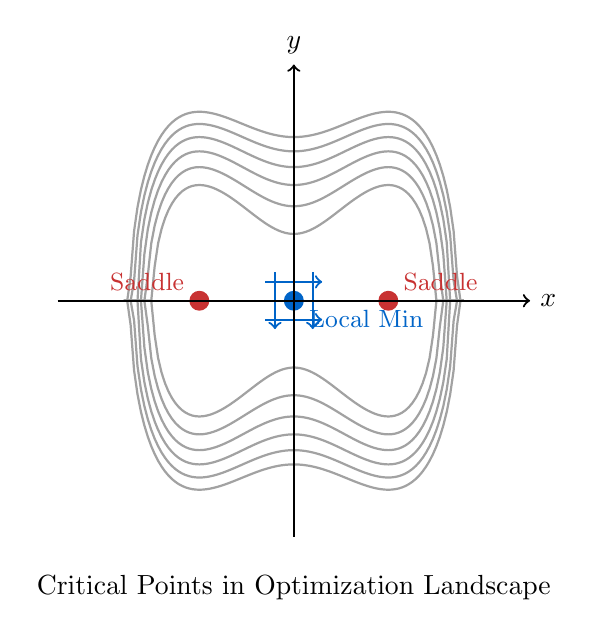
\begin{tikzpicture}[scale=1.2]
  % Define colors
  \definecolor{mincolor}{RGB}{0,100,200}
  \definecolor{saddlecolor}{RGB}{200,50,50}
  \definecolor{contourcolor}{RGB}{100,100,100}
  
  % Draw contour lines for the function f(x,y) = x^4 - 2x^2 + y^2
  \foreach \level in {0.5,1.0,1.5,2.0,2.5,3.0} {
    \draw[contourcolor!60, thick] plot[domain=-1.8:1.8, samples=100] (\x, {sqrt(max(0,\level - \x*\x*\x*\x + 2*\x*\x))});
    \draw[contourcolor!60, thick] plot[domain=-1.8:1.8, samples=100] (\x, {-sqrt(max(0,\level - \x*\x*\x*\x + 2*\x*\x))});
  }
  
  % Mark critical points
  % Local minimum at (0,0)
  \fill[mincolor] (0,0) circle (3pt) node[below right, xshift=2pt] {\small Local Min};
  
  % Saddle points at (±1,0)
  \fill[saddlecolor] (1,0) circle (3pt) node[above right, xshift=2pt] {\small Saddle};
  \fill[saddlecolor] (-1,0) circle (3pt) node[above left, xshift=-2pt] {\small Saddle};
  
  % Add arrows showing gradient directions
  \draw[->, mincolor, thick] (-0.3,0.2) -- (0.3,0.2);
  \draw[->, mincolor, thick] (-0.3,-0.2) -- (0.3,-0.2);
  \draw[->, mincolor, thick] (0.2,0.3) -- (0.2,-0.3);
  \draw[->, mincolor, thick] (-0.2,0.3) -- (-0.2,-0.3);
  
  % Add coordinate axes
  \draw[->, black, thick] (-2.5,0) -- (2.5,0) node[right] {$x$};
  \draw[->, black, thick] (0,-2.5) -- (0,2.5) node[above] {$y$};
  
  % Add labels
  \node[below] at (0,-2.8) {Critical Points in Optimization Landscape};
\end{tikzpicture}
\caption{Visualization of critical points in the function $f(x,y) = x^4 - 2x^2 + y^2$. The local minimum at $(0,0)$ shows converging gradient directions, while saddle points at $(\pm 1,0)$ demonstrate mixed curvature with both converging and diverging directions.}
\label{fig:critical-points}
\end{figure}

The function $f(x,y) = x^4 - 2x^2 + y^2$ demonstrates three distinct types of critical points that commonly appear in optimization landscapes. At the local minimum $(0,0)$, the function value $f(0,0) = 0$ represents the lowest point in the neighborhood, with all nearby points having higher function values. The gradient vanishes at this point, and the Hessian matrix has positive eigenvalues, indicating concave-up curvature in all directions.

Saddle points at $(\pm 1,0)$ represent the most challenging critical points for optimization, where $f(\pm 1,0) = -1$ creates deceptive flat regions. These points have zero gradients but mixed curvature, with the Hessian containing both positive and negative eigenvalues. This mixed curvature means that while some directions lead downhill, others lead uphill, creating a complex landscape where gradient descent can become trapped.

In high-dimensional optimization, saddle points are much more common than local minima, making them the primary challenge for gradient-based methods. The visualization clearly shows how saddle points create deceptive flat regions where optimization can stall, while local minima provide clear convergence targets.

\subsection{Plateaus}\index{plateau}

Flat regions with small gradients slow convergence. Adaptive methods and learning rate schedules help navigate plateaus.

\subsection{Practical Optimization Strategy}

Developing an effective optimization strategy requires understanding the interplay between optimizer choice, learning rate scheduling, and problem-specific considerations. The recommended approach begins with Adam for rapid initial progress, using learning rates in the range $\{10^{-3},3\cdot10^{-4},10^{-4}\}$ to establish a strong foundation for training. This adaptive method provides robust performance across diverse architectures and datasets while requiring minimal hyperparameter tuning.

Learning rate scheduling plays a crucial role in optimization success, with different strategies suited to different model architectures. Cosine decay with warmup proves particularly effective for transformer-like models, providing smooth transitions from exploration to exploitation phases. For convolutional networks trained with SGD and momentum, step decay schedules often yield superior results by allowing the optimizer to make large initial progress before fine-tuning with smaller learning rates.

When validation accuracy saturates, switching from Adam to SGD with Nesterov momentum can improve generalization by providing different optimization dynamics. This transition requires careful tuning of both learning rate and momentum parameters, but often yields better final performance on vision tasks. Gradient clipping becomes essential in recurrent models and unstable training scenarios, preventing parameter updates from becoming too large while preserving optimization direction.

Continuous monitoring of training and validation metrics provides essential feedback for optimization strategy adjustment. Early stopping prevents overfitting by halting training when validation performance plateaus, while careful attention to learning rate schedules ensures optimal convergence behavior throughout the training process.\index{gradient clipping}\index{early stopping}

Applications and heuristics:
\begin{itemize}
    \item Vision: SGD+momentum or Nesterov often yields state-of-the-art with careful schedules and augmentations \cite{He2016}.
    \item NLP/Transformers: Adam/AdamW with warmup+cosine is a strong default; clip global norm in seq2seq models.
    \item Reinforcement learning: Adam with small $\alpha$ stabilizes non-stationary objectives.
\end{itemize}

Common failure modes:
\begin{itemize}
    \item Divergence at start: reduce $\alpha$, add warmup, or increase \(\epsilon\) for Adam.
    \item Plateau: try larger batch with warmup, use cosine schedule, or add momentum.
    \item Overfitting: increase regularization (weight decay, dropout), add data augmentation.
\end{itemize}

% Chapter 8, Section 6

\section{Key Takeaways \difficultyInline{intermediate}}
\label{sec:ch8-key-takeaways}

\begin{keytakeaways}
\begin{itemize}
    \item \textbf{Mini-batch SGD is the workhorse:} balances speed and stability; pair with momentum and schedules.
    \item \textbf{Momentum and Nesterov reduce oscillations:} accelerate along consistent directions and dampen noise.
    \item \textbf{Adaptive methods ease tuning:} Adam often works out-of-the-box; consider switching to SGD+momentum late for best generalisation.
    \item \textbf{Curvature matters:} second-order ideas inspire preconditioning; full Hessians are usually impractical in deep nets.
    \item \textbf{Schedules are critical:} cosine or step decay often yield large gains; warmup stabilises early training.
    \item \textbf{Mitigate pathologies:} use proper initialisation, normalisation, and gradient clipping to handle vanishing/exploding gradients and plateaus.
\end{itemize}
\end{keytakeaways}

% Index entries
\index{optimisation!key takeaways}



% % Chapter 8: Real World Applications

\section{Real World Applications}
\label{sec:optimization-real-world}


Optimization techniques are the engine that makes deep learning work in practice. Without effective optimization, even the best model architectures would fail to learn. Here's how optimization impacts real-world systems.

\subsection{Training Large Language Models}

Modern AI assistants rely on advanced optimization for their capabilities:

\begin{itemize}
    \item \textbf{Training ChatGPT and similar models:} These models contain billions of parameters and require months of training on thousands of GPUs. Advanced optimizers like Adam with learning rate schedules make this computationally feasible. Without proper optimization, training would take years or fail to converge entirely.
    
    \item \textbf{Managing computational costs:} Training large models costs millions of dollars in electricity and computing time. Efficient optimization techniques like gradient accumulation and mixed-precision training reduce these costs by 50\% or more, making advanced AI accessible to more organizations.
    
    \item \textbf{Fine-tuning for specific tasks:} When adapting a pre-trained model for specific applications (like legal document analysis or medical question answering), careful optimization allows effective adaptation with just hours of training instead of starting from scratch.
\end{itemize}

\subsection{Real-Time Computer Vision}

Vision systems in phones, security cameras, and robots depend on optimization:

\begin{itemize}
    \item \textbf{Smartphone facial recognition:} Your phone unlocks in a fraction of a second by running an optimized neural network. The model was trained using techniques like momentum and learning rate decay to achieve high accuracy with a small enough network to run on battery-powered devices.
    
    \item \textbf{Video surveillance systems:} Security systems process multiple camera feeds simultaneously, detecting unusual activities in real-time. Optimization techniques enable training models that are both accurate and fast enough to analyze video streams without delays.
    
    \item \textbf{Augmented reality applications:} AR effects on social media apps track faces and objects in real-time at 60 frames per second. This requires models optimized for both accuracy and speed, achieved through careful training with modern optimization methods.
\end{itemize}

\subsection{Recommendation Systems at Scale}

Online platforms serve personalized content to billions of users:

\begin{itemize}
    \item \textbf{YouTube video recommendations:} YouTube's recommendation system processes viewing patterns from billions of users and millions of videos. Advanced optimization techniques like distributed training across data centers make it possible to update these models daily, ensuring recommendations stay fresh and relevant.
    
    \item \textbf{News feed personalization:} Social media platforms continuously optimize models to show you content you'll find engaging. The system needs to learn quickly from your recent interactions while balancing exploration (showing new content) and exploitation (showing what you've liked before).
    
    \item \textbf{E-commerce product matching:} Online retailers optimize models to match products with potential buyers. The optimization must balance multiple objectives: conversion rates, customer satisfaction, inventory levels, and profit margins, all while training on constantly changing data.
\end{itemize}

\subsection{Why Optimization Matters}

The impact of good optimization in real applications:
\begin{itemize}
    \item \textbf{Speed:} Faster training means quicker iteration and deployment
    \item \textbf{Cost:} Efficient optimization reduces computational expenses dramatically
    \item \textbf{Quality:} Better optimization leads to more accurate models
    \item \textbf{Feasibility:} Some applications only become possible with advanced optimization
\end{itemize}

Optimization is where theory meets practice—the techniques in this chapter determine whether ambitious deep learning projects succeed or fail in the real world.

% Index entries
\index{applications!language models}
\index{applications!computer vision}
\index{applications!recommendation systems}
\index{optimization!applications}

% % Chapter 8, Section 7

\section{Problems \difficultyInline{intermediate}}
\label{sec:ch8-problems}

This section provides exercises to reinforce your understanding of optimization. Problems are categorized by difficulty and include hints.

\subsection{Easy Problems (6 problems)}

\begin{problem}[Batch vs. Mini-batch]
List two pros and two cons of batch GD vs. mini-batch SGD for large-scale training.

\textbf{Hint:} Consider gradient variance, compute efficiency, and convergence behavior.
\end{problem}

\begin{problem}[Learning Rate Intuition]
Describe qualitatively what happens if the learning rate is too small or too large.

\textbf{Hint:} Look for slow progress vs. divergence/oscillation.
\end{problem}

\begin{problem}[Momentum Update]
Write the momentum update for parameters and explain the role of $\beta$.

\textbf{Hint:} Velocity accumulates an EMA of past gradients.
\end{problem}

\begin{problem}[AdaGrad Scaling]
Explain why AdaGrad reduces step sizes over time and when this helps.

\textbf{Hint:} Accumulated squared gradients grow; sparse features benefit.
\end{problem}

\begin{problem}[Adam Defaults]
State Adam's common default hyperparameters and what each controls.

\textbf{Hint:} $\beta_1,\beta_2,\epsilon,\alpha$.
\end{problem}

\begin{problem}[Gradient Clipping]
Give a reason to clip gradients and one potential downside.

\textbf{Hint:} Stabilization vs. biasing the update direction.
\end{problem}

\subsection{Medium Problems (5 problems)}

\begin{problem}[Nesterov Look-ahead]
Derive the Nesterov update by evaluating the gradient at the look-ahead point and compare to classical momentum.

\textbf{Hint:} Replace $\nabla L(\theta_t)$ by $\nabla L(\theta_t+\beta v_{t-1})$.
\end{problem}

\begin{problem}[RMSProp vs. AdaGrad]
Show how RMSProp's EMA avoids AdaGrad's overly aggressive decay and discuss hyperparameter $\rho$.

\textbf{Hint:} Replace cumulative sum with exponential moving average.
\end{problem}

\begin{problem}[Adam Bias Correction]
Derive the bias-corrected moments $\hat m_t, \hat v_t$ and explain why correction matters early in training.

\textbf{Hint:} Compute $\mathbb{E}[m_t]$ under zero initialization.
\end{problem}

\begin{problem}[Plateaus and Schedules]
Explain why cosine annealing or step decay can help escape plateaus compared to a fixed learning rate.

\textbf{Hint:} Larger steps at the right time.
\end{problem}

\begin{problem}[L-BFGS Memory]
Describe how L-BFGS maintains a low-rank inverse Hessian approximation using recent curvature pairs.

\textbf{Hint:} Limited history of $(s_t, y_t)$ updates.
\end{problem}

\subsection{Hard Problems (5 problems)}

\begin{problem}[Natural Gradient Rationale]
Argue why the Fisher information provides a geometry suited for probabilistic models and yields reparameterization-invariant updates.

\textbf{Hint:} Consider KL divergence as the local distance measure.
\end{problem}

\begin{problem}[Saddle Points in High Dimensions]
Provide an argument for why saddle points are more prevalent than local minima in high-dimensional non-convex problems.

\textbf{Hint:} Random matrix spectra and sign patterns of eigenvalues.
\end{problem}

\begin{problem}[Warmup Heuristics]
Justify learning rate warmup in the presence of normalization layers and large batch sizes.

\textbf{Hint:} Stabilize early updates before full-strength steps.
\end{problem}

\begin{problem}[SGD vs. Adam Generalization]
Discuss hypotheses for why SGD with momentum can outperform Adam on final generalization despite slower early progress.

\textbf{Hint:} Implicit regularization and noise structure.
\end{problem}

\begin{problem}[Design an Optimization Plan]
For training a ResNet-50 on a new 100-class dataset, propose an end-to-end optimization plan (initializer, optimizer, schedule, batch size, clipping, regularization) and justify choices.

\textbf{Hint:} Consider compute budget, stability, and expected generalization.
\end{problem}

% Index entries
\index{problems!optimization}
\index{exercises!optimization}




% Chapter exercises
% Exercises (Hands-On Exercises) for Chapter 8: Optimization for Training Deep Models

\section*{Exercises}
\addcontentsline{toc}{section}{Exercises}

\subsection*{Easy}

\begin{exercisebox}[easy]
\begin{problem}[Batch Size Selection]
Explain the trade-offs between using a large batch size versus a small batch size for training. Consider computation time, memory usage, and convergence properties.
\end{problem}
\begin{hintbox}
Think about GPU utilization, gradient noise, and generalization gap.
\end{hintbox}
\end{exercisebox}


\begin{exercisebox}[easy]
\begin{problem}[Momentum Intuition]
Describe how momentum helps accelerate optimization. Use the analogy of a ball rolling down a hill to explain the concept.
\end{problem}
\begin{hintbox}
Consider how previous gradients influence the current update and help overcome small local variations.
\end{hintbox}
\end{exercisebox}


\begin{exercisebox}[easy]
\begin{problem}[Learning Rate Scheduling]
List three common learning rate scheduling strategies and explain when each is most appropriate.
\end{problem}
\begin{hintbox}
Consider step decay, exponential decay, cosine annealing, and cyclical learning rates.
\end{hintbox}
\end{exercisebox}


\begin{exercisebox}[easy]
\begin{problem}[Adam Hyperparameters]
Adam optimizer has hyperparameters $\beta_1$ (typically 0.9) and $\beta_2$ (typically 0.999). Explain the role of each parameter.
\end{problem}
\begin{hintbox}
$\beta_1$ controls momentum (first moment), $\beta_2$ controls adaptive learning rates (second moment).
\end{hintbox}
\end{exercisebox}


\subsection*{Medium}

\begin{exercisebox}[medium]
\begin{problem}[Optimizer Comparison]
Compare SGD with momentum, RMSProp, and Adam on a simple optimization problem. Discuss their convergence behavior and when to prefer one over another.
\end{problem}
\begin{hintbox}
Consider sparse gradients, non-stationary objectives, and computational cost.
\end{hintbox}
\end{exercisebox}


\begin{exercisebox}[medium]
\begin{problem}[Gradient Clipping]
Explain why gradient clipping is important for training recurrent neural networks. Derive the gradient clipping formula and discuss the choice of threshold.
\end{problem}
\begin{hintbox}
Consider exploding gradients and the norm $\|\nabla L\|$. Clip by value or by norm.
\end{hintbox}
\end{exercisebox}


\subsection*{Hard}

\begin{exercisebox}[hard]
\begin{problem}[Natural Gradient Descent]
Derive the natural gradient update rule and explain why it is invariant to reparameterisations. Discuss the computational challenges of using natural gradient in deep learning.
\end{problem}
\begin{hintbox}
Consider the Fisher information matrix $\mat{F}$ and the update $\boldsymbol{\theta} \leftarrow \boldsymbol{\theta} - \eta \mat{F}^{-1} \nabla L$.
\end{hintbox}
\end{exercisebox}


\begin{exercisebox}[hard]
\begin{problem}[Learning Rate Warmup]
Analyse why learning rate warmup is beneficial when training with large batch sizes. Provide theoretical justification based on the optimization landscape.
\end{problem}
\begin{hintbox}
Consider the stability of gradients in early training and the sharpness of the loss landscape.
\end{hintbox}
\end{exercisebox}


\begin{exercisebox}[hard]
\begin{problem}[Optimizer Comparison]
Compare the convergence properties of SGD, Adam, and RMSprop on a non-convex optimization problem.
\end{problem}
\begin{hintbox}
Consider the adaptive learning rates and momentum effects of each optimizer.
\end{hintbox}
\end{exercisebox}


\begin{exercisebox}[hard]
\begin{problem}[Gradient Clipping]
Explain when and why gradient clipping is necessary. How does it affect the optimization dynamics?
\end{problem}
\begin{hintbox}
Consider the exploding gradient problem and the relationship between gradient norms and learning stability.
\end{hintbox}
\end{exercisebox}


\begin{exercisebox}[hard]
\begin{problem}[Learning Rate Scheduling]
Design a learning rate schedule for training a deep network. Compare step decay, exponential decay, and cosine annealing.
\end{problem}
\begin{hintbox}
Consider the trade-off between exploration and exploitation in different phases of training.
\end{hintbox}
\end{exercisebox}


\begin{exercisebox}[hard]
\begin{problem}[Second-Order Methods]
Explain why second-order optimization methods are rarely used in deep learning despite their theoretical advantages.
\end{problem}
\begin{hintbox}
Consider computational complexity, memory requirements, and the stochastic nature of deep learning.
\end{hintbox}
\end{exercisebox}


\begin{exercisebox}[hard]
\begin{problem}[Optimization Landscape]
Analyse the relationship between the optimization landscape and the choice of optimizer for deep networks.
\end{problem}
\begin{hintbox}
Consider saddle points, local minima, and the role of noise in optimization.
\end{hintbox}
\end{exercisebox}


\begin{exercisebox}[hard]
\begin{problem}[Batch Size Effects]
Investigate how batch size affects optimization dynamics and generalization in deep learning.
\end{problem}
\begin{hintbox}
Consider the relationship between batch size, gradient noise, and the implicit regularization effect.
\end{hintbox}
\end{exercisebox}



